\documentclass{article}
% V1 workshop short (ML4PS / NeurReps class) paper. Canonical content: draft.md.
% Standard-package build; compiles with pdflatex or tectonic. Author block anonymized.
\PassOptionsToPackage{round}{natbib}
\usepackage[dblblindworkshop]{neurips_2026}
\usepackage[utf8]{inputenc}
\usepackage[T1]{fontenc}
\usepackage{amsmath,amssymb,amsthm}
\usepackage{amsfonts}
\usepackage{booktabs}
\usepackage{graphicx}
\usepackage{microtype}
\usepackage{bm}
\usepackage[hidelinks]{hyperref}
\usepackage{url}
\usepackage{xcolor}

\newcommand{\R}{\mathbb{R}}
\newcommand{\half}{\tfrac12}
\newcommand{\detJ}{\det J}

\title{Certified Access: Test-Time Compute on a Conservative Physics-Structured AI Memory}
\author{[AUTHORS PLACEHOLDER]}
\date{}

\begin{document}
\sloppy
\maketitle

\begin{abstract}
Test-time compute mechanisms, such as retries, confidence-based escalation, and non-local routing, are conventionally deployed as black-box augmentations to trained models. These approaches typically introduce additional forward passes or learned halting heads without providing a structural account of the specific capabilities acquired by the additional compute, nor do they quantify the costs incurred against the model's fundamental stability guarantees. In this work, we propose a theoretical and empirical framework for certified access in causal, symplectic associative memories. When the underlying latent state $(q,p)$ is advanced by a damped symplectic (velocity-Verlet) step of a learned Hamiltonian, every compute mechanism that expands access has an exact phase-volume Jacobian, a bounded energy change, and an exact latch-transport law. We formalize latent reachability into two distinct failure modes. First, escape failures occur within $C_T$ when a state is trapped behind latent surface barrier. Second, reach failures occur when a target lies outside a kinematic causal box $C_T$. To resolve escape failures, we deploy a Lorentz squeeze, which injects bounded, re-absorbable energy that expands reach at test time. To resolve reach failures, we introduce a gated canonical translation (a one-step channel across $C_T$), which expands latent reach at $\detJ=1$ exactly. We verify this certificate stack on a designed analytic testbed, and show that reaching just beyond $C_T$ with the squeeze requires energy growing quadratically in the excess distance covered, whereas the gated channel's energy requirement is fixed and independent of distance. Furthermore, we separate transport from latent state-replacement, demonstrating that an untrained state-replacing map annihilates phase volume and erases stored charge, while the gated channel preserves it. Finally, we situate these mechanisms on a learned physics-structured memory, demonstrating memory-agnostic calibrated compute-rationing and evaluating scaling boundaries for non-local routing against a physics-free baseline. The primary contribution of this work lies in the theoretical formalization and empirical verification of the certificate stack, prioritizing structural discipline over isolated benchmark performance.
\end{abstract}

\section{Introduction}
Current deep learning architectures increasingly rely on adaptive test-time compute to dynamically allocate inference budgets. Approaches such as learned halting (ACT, \citealp{graves_adaptive_2017}; PonderNet, \citealp{banino_pondernet_2021}), confidence-gated early exits (CALM, \citealp{schuster_confident_2022}), learned routing (Mixture-of-Depths, \citealp{raposo_mixture--depths_2024}; Mixture-of-Experts, \citealp{shazeer_outrageously_2017}), and energy-based verification \citep{gladstone_energy-based_2025} have established the utility of input-conditional escalation. However, these mechanisms generally bolt a learned scalar gate onto a feedforward stack. Consequently, escalating compute merely replicates the standard forward operation without providing a structural guarantee of how the additional computation explicitly alters the latent state of the model.

To resolve this limitation, we introduce a framework that defines test-time compute for Latent Dynamics Models (the class of algorithms that explicitly structures the dynamics of abstract latent spaces parametrized by some encoder). If the queried memory is a conservative latent state $(q,p)$ (generated by the encoder) advanced by a structure-preserving symplectic integrator of a learned separable Hamiltonian $H(q,p)=T(p)+V_\theta(q)$ (of the latent space produced by any encoder, not limited to a Hamiltonian describing the input space/system), test-time compute manifests as access to a defined phase space during inference. Here the kinetic term is formulated by a causal relativistic governor as in~\citet{jawahar_chlu_2026}. Within this regime, the physical properties of the phase space strictly define every access mechanism. We formalize this paradigm as certified access, where each mechanism is accompanied by a physical certificate.

This certificate comprises of three components: the Jacobian determinant $\detJ$ (to certify phase volume conservation), a bounded energy change (to quantify injected energy), and a latch-transport law (to determine the transformation of content stored in protected continuous-symmetry directions). Crucially, these certificates are verifiable theorems derived from the underlying symplectic structure rather than empirical curves fit to specific datasets. We state each certificate as a theorem and verify it on a designed testbed: the exactness claims ($\det J$, the energy change and the latch-transport law) hold to machine precision, while the re-absorption and channel-hop thresholds are verified to leading order.

\section{Setup: A Conservative Memory and its Reachable Set}
\paragraph{Reference architecture and terminology:}
The reference memory presented here is the Causal Learning Unit (CLU), introduced as CHLU in \citet{jawahar_chlu_2026}. The empirical results in this work assume the reference training objective of the CLU but evaluate generalized properties of the learned Hamiltonian.

\paragraph{The governed map:}
The CLU is a unit where a discrete latent state $(q,p)$, produced by some encoder, is advanced by one dissipative velocity-Verlet~\citep{martys1999velocity} step with size $\varepsilon$ and per-step damping $\gamma\in[0,1)$. This constitutes a kick-drift-kick integration of the separable Hamiltonian $H=T(p)+V_\theta(q)$, followed by momentum scaling $p\mapsto(1-\gamma)p$. This update is conformally symplectic, adhering to $J^\top\Omega J=(1-\gamma)\Omega$ and yielding $\detJ=(1-\gamma)^d$ in $d$-dimensions. The relativistic kinetic mode enforces a strict cap on velocity, defined as $|\dot q_i|<c/\sqrt{M_i}$, where $c$ is a hyper-parameter. To bleed excess energy toward a target $E^\star$, a state-dependent governor $\gamma_n=s\tanh(\max(0,H-E^\star))$ is applied. Derivations and validations are provided in App.~\ref{app:deriv}.

\paragraph{Latent reachability constraints:}
For the governed map $\Phi_{\varepsilon,\gamma}$, the $T$-step reachable set originating from $z_0$ is defined as $R_T(z_0)=\{\Phi^n(z_0):1\le n\le T\}$, with its position shadow denoted as $Q_T(z_0)$. To successfully access a latent memory state, the underlying mechanism must strictly enlarge $Q_T$. App.~\ref{app:deriv:box} proves that a single drift step advances position $q$ by at most $\varepsilon c/\sqrt{M_i}$ per coordinate. Consequently, the reachable set is strictly bounded:
\[
Q_T(z_0)\ \subseteq\ C_T(q_0):=\{q:\ |q_i-q_{0,i}|\le L_i,\ L_i=T\varepsilon c/\sqrt{M_i}\}.
\]
The resulting causal box $C_T$ is entirely energy-blind, as injected momentum asymptotically approaches, but cannot exceed, the velocity limit $c/\sqrt{M_i}$ (App.~\ref{app:deriv:box}).

\paragraph{Failure modes:} In this setup there are two main failure modes \emph{Kinematic Reach} and \emph{Energetic Escapes}. Kinematic reach failures occur when the target $q^\star\notin C_T(q_0)$, a condition solvable only by a non-local jump. Energetic escape failures occur when the target $q^\star\in C_T(q_0)$ but is shielded by a potential barrier $\Delta V_b$ that the latent energy cannot traverse. This is resolved by any bounded energy injection that acts faster than the governor can dissipate it.

\section{Mechanism Certificates and Limitations}
\paragraph{Escape resolution via Lorentz squeeze:}
To solve energetic escape failure, we apply a mass-weighted Lorentz squeeze $S^{(M)}_\zeta$ \citep{wales_global_1997}. This map is exactly symplectic ($\det=1$) and amplifies velocity and displacement toward the saddle according to $\delta q'=\delta q\cosh\zeta+p_0\sinh\zeta$, where $\zeta$ is the rapidity or the squeeze strength. The injected energy is strictly bounded by $H(S_\zeta z)\le e^{2|\zeta|}H(z)$ (Appendix~\ref{app:deriv:squeeze}), and the internal governor dissipates the excess in approximately $2\zeta/\gamma_c$ steps. We evaluate this on a matched quadratic potential, confirming that the energy injection accurately tracks the theoretical bound across varying rapidities listed in App.~\ref{app:res}.

\paragraph{Reach resolution via intra-unit gated-channels:}
To solve kinematic reach failure, we introduce an intra-unit \emph{gated channel} defined by a learned pair of loci $(a,b)$ governed by a hard gate frozen at capture. This applies a constant canonical translation $q\mapsto q+\Delta,\ p\mapsto p$, where $\Delta=b-a$. Because this mechanism mirrors the flow of the linear Hamiltonian $W=\Delta\cdot p/\tau$, the Jacobian is the identity matrix $I_{2d}$, yielding $\detJ=1$ exactly. This property remains independent of $\Delta$ and the gate itself. The energy required is a discrete jump $\Delta H_{\rm wh}=V_\theta(q+\Delta)-V_\theta(q)$ that must be tracked explicitly, where matched loci result in transport at zero energy. Brief evaluation listed in App.~\ref{app:res}. As a necessary design guard, if a gate varies dynamically during the jump, the volume preservation is broken by an uncompensated contraction ($\detJ=1+\nabla g\cdot\Delta\neq1$, measured at 2.05 in unit testing).

\paragraph{Latch transport law:}
For a protected direction maintaining an invariant parameter $Q=p^\top X q$ (also called the Goldstone charge, borrowing from field theory along the lines of~\citet{iqbal_spontaneous_2026}), where $X$ is the symmetry broken generator, the channel shift exactly evaluates to $Q'-Q=p^\top X\Delta$. Because the gated channel maps a single phase point, it transports the latch rather than copying or erasing it.

\paragraph{BIBO stability limitations:}
The certificate $\detJ=1$ guarantees volume preservation but does not guarantee trajectory boundedness. If a channel exit is placed outside the coercive connected component of the potential $V_\theta$, the trajectory can escape to infinity, even if the jump is symplectic and the energy change is exactly zero. Evaluated on a controlled non-coercive potential ($V=\half kq_0^2-\epsilon q_0^4$), an exit at $b=5.0$ requires zero energy ($\Delta H=0.0$ exactly) and passes an energy-only sub-level test, yet the trajectory escapes with a growth rate proportional to the temporal horizon ($r^\ast\propto T$). In contrast, an admissible exit at $b=3.0$ requires an energy change of $\Delta H=2.88$ but remains bounded (see Fig.~\ref{fig:bibo}). Therefore, membership in the coercive component is the mandatory operational clause for BIBO stability. The full certificate parameters are detailed in Appendix B.

\subsection{Differentiating Access Mechanisms}
\label{sec:testbed}
To systematically analyze these reachability bounds, we construct a controlled reach battery across a $K$-basin double well with barriers spanning across the causal box $L=2.5$ ($T=100$, $\varepsilon=0.05$, $c=1$, heavy reach coordinate $M_0=4.0$). The governor is parameterized such that plain relaxation is mathematically blocked from escaping (kinetic energy $0.72 < \Delta V_b=1$). We measure the landing rates across distances $d<L=\{0.8,1.6,2.4\}$ and $d>L=\{3.2,4.0,5.0\}$.

\begin{center}\footnotesize
\begin{tabular}{lccll}
\toprule
Algorithm & $d{<}L$ & $d{>}L$ & Measured $\detJ$ & Diagnostic \\
\midrule
Plain relaxation & $0$ & $0$ & $(1{-}\gamma)^d$ & Completely escape-blocked \\
Squeeze $S^{(M)}$ & $1$ & $\to0$ & $1.000\pm4\mathrm{e}{-6}$ & Reach beyond $C_T$ needs energy $\le e^{2|\zeta|}H$ \\
Gated channel & $1$ & $1$ & $1.0$ exact & Flat access scaling; exact $0.0$ energy change \\
Newtonian control & $1$ & $1$ & $1.0$ & Confirms relativistic cap bounds flow \\
State-replacing map & $1$ & $1$ & $0.0$ exact & State overwritten; volume annihilated \\
Dense/$V$-throat & $\to0$ & $0$ & $(1{-}\gamma)^d$ & Modulates barrier; fails global reach \\
\bottomrule
\end{tabular}
\end{center}

The squeeze mechanism extends the reach bound to $[L,\,L+p_0\sinh\zeta/M_0]$ (shaded region in Fig.~\ref{fig:reach}(a)). However, because the energy scales as $e^{2|\zeta|}H$, reaching $d=4.0$ analytically requires $\zeta\approx2.01$, and $d=5.0$ requires $\zeta\approx2.64$. Consequently, reach via squeeze requires energy growing exponentially in rapidity $\zeta$ and therefore quadratically in the excess distance, whereas the gated channel's (gated channel's) energy requirement is fixed and independent of distance as shown in Fig.~\ref{fig:reach}(a). The squeeze failing to reach the outer distances simply indicates that the energy it requires exceeds the swept rapidity budget ($\zeta\le2.0$), not that it is fundamentally incapable of reaching them if provided sufficient energy. Notably, the untrained state-replacing map ($(q,p)\mapsto(b,p)$) demonstrates an identical landing rate to the gated channel. However, its Jacobian is mathematically block-diagonal with zero blocks, yielding $\detJ=0$ exactly, as measured by forward-mode automatic differentiation. This map is volume-annihilating and non-invertible, erasing the state completely. The Newtonian control successfully reaches past the box, confirming that the relativistic causal cap governs the primary flow limitation. Plain relaxation is escape-blocked across all distances.

\begin{figure}[htb!]
\centering
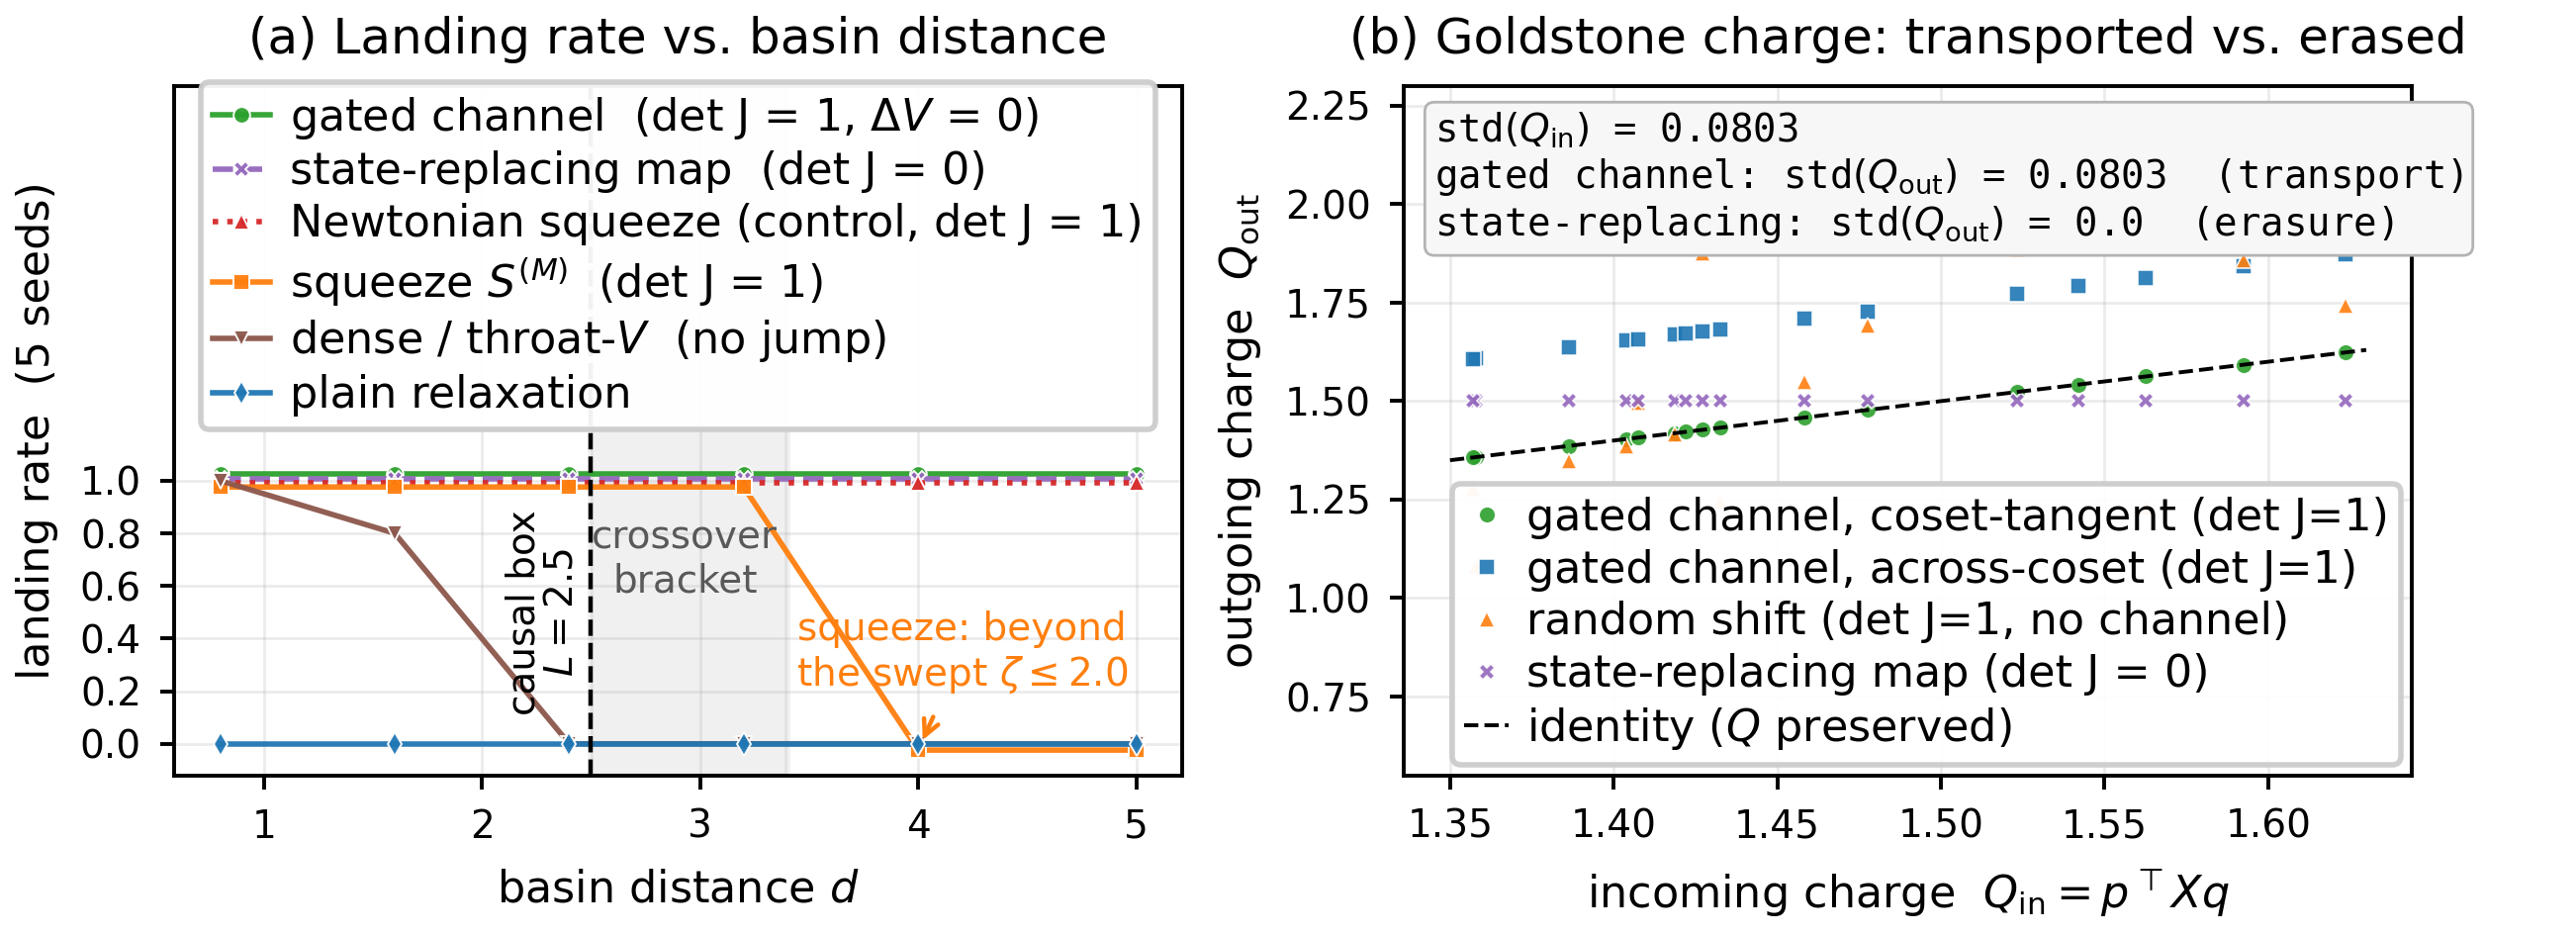
\includegraphics[width=\textwidth]{figs/fig1_certificate.png}
\caption{\textbf{Verification of the certificate stack on the designed testbed (Sec.~\ref{sec:testbed}). (a) Reach capabilities:} Landing rate as a function of basin distance $d$ evaluated on a symmetric double-well potential (dim 2, 5 seeds, $L=2.5$). \textbf{(b) The certificate in force:} Comparison of outgoing versus incoming Goldstone charge for 16 sample states drawn from the capture ball.}
\label{fig:reach}
\end{figure}


\subsubsection{The Certificate's Consequence: State Erasure vs. Transport}
\label{sec:erasure}
To evaluate the downstream consequence of the $\detJ$ certificates, we track a cloud of 16 initial states drawn uniformly from the capture ball ($\mathrm{std}(Q_{\rm in})=0.0803$). It is critical to distinguish between an analytic transport map and a learned decision head. A learned decision router may select whether to utilize a non-local edge, but it transports the data through the certified $\detJ=1$ gated channel channel. The object evaluated here is a pure, untrained state-replacing map that physically overwrites the state.

\paragraph{The transport guarantee:}
The canonical translation of the gated channel (gated channel) is injective, shifting every incoming state's charge by the exact constant $p^\top X\Delta$ ($\max\text{error}\le1.2\times10^{-7}$). The topological spread is strictly preserved ($\mathrm{std}(Q_{\rm out})=0.0803$) as shown in Fig.~\ref{fig:reach}(b), and the pre-jump state remains exactly recoverable  ($q_{\rm in}=q_{\rm out}-\Delta$, max err $2.2{\times}10^{-8}$). Results tabulated in App.~\ref{app:res}.

Conversely, the state-replacing map ($\detJ=0$) maps all 16 distinct states onto a singular bit-identical charge ($\mathrm{std}(Q_{\rm out})=0$). The coset content is irreversibly erased. This demonstrates a mechanism-level violation on a designed testbed, establishing that at $\detJ=1$, the matched canonical channel transports the stored charge, while a $\detJ=0$ state-replacing jump erases it. We explicitly note that volume preservation alone is not the latch certificate, as the random-shift baseline maintains $\detJ=1$ but still scrambles the topological spread. The matched channel preserves it.

\section{Translating Mechanisms to Learned Memories}
To determine the practical viability of these formalisms, we evaluate three applications on trained associative memories. We transition from the analytic testbed to learned configurations, strictly tracking the energy required by every mechanism and establishing boundaries where baseline heuristics outperform our proposed approach.

\subsection{Memory-Agnostic Calibrated Compute-Rationing}
\label{sec:rationing}
We implement a self-calibrating gating mechanism on a trained CLU associative memory configured for MQAR key-value recall (vocab 256, capacity limits kv$\in\{16,24,32\}$, 5 seeds). We apply a Learn-then-Test (LTT; \citealp{angelopoulos_learn_2025}) wrapper to determine exit thresholds based on a dynamic relaxation ladder \citep{geifman_selective_2017}.
\begin{enumerate}\itemsep2pt
    \item \textbf{Uniform transfer of calibration:} The identical calibration stack applied to a baseline modern Hopfield memory \citep{ramsauer_hopfield_2021} yields analogous improvements (raw $0.18\to$ calibrated $0.88$, matching the CLU's $0.43\to0.87$). The gating mechanism is therefore memory-agnostic; we do not assert that the CLU possesses an inherently superior energy signal.
    \item \textbf{Escalatable rationing impacts low-capacity regimes:} At an under-converged 400-epoch training budget, the memory demonstrates a $4.81\pm0.44\times$ step-reduction at the kv16 capacity level compared to an always-full relaxation budget, while achieving a higher accuracy (Fig.~\ref{fig:frontier}). This efficiency gain decays as capacity demands scale, yielding $1.57\pm0.07\times$ at kv24, and $1.14\pm0.06\times$ at kv32. At full convergence (2000 epochs), the gating mechanism achieves strict parity with the full-budget baseline rather than exceeding it. Therefore, the core asset of the gate is compute rationing on clean retrieval tasks, not generalized accuracy dominance.
\end{enumerate}

We map the same gate across capacity and training budget on a 198-job evaluation grid (Fig.~\ref{fig:frontier}). Storage fidelity converges to near-perfect levels across training epochs, indicating that the initial underperformance was an under-training artifact. Performance degradation beyond kv64 is constrained by epoch-budgets rather than hard capacity limits; training models to 4000 epochs, however, causes smaller cells to over-train, degrading accuracy from $1.00$ to $0.89$. The measured step-reductions of the CLU gate ($9.9\times, 9.5\times, 6.2\times$ across kv32, kv64, kv96) represent intra-CLU rationing against a full-budget CLU baseline. Under evaluation cue noise ($\sigma\in\{0.3,0.6\}$), the gate degrades sharply: at $\sigma=0.6$ on kv32, the CLU gate yields an accuracy of $0.36$, despite underlying CLU storage fidelity remaining at $1.0$. The governed relaxation over-commits to the corrupted cue, and we record this noise wall as an open problem.

\begin{figure}[htb!]\centering
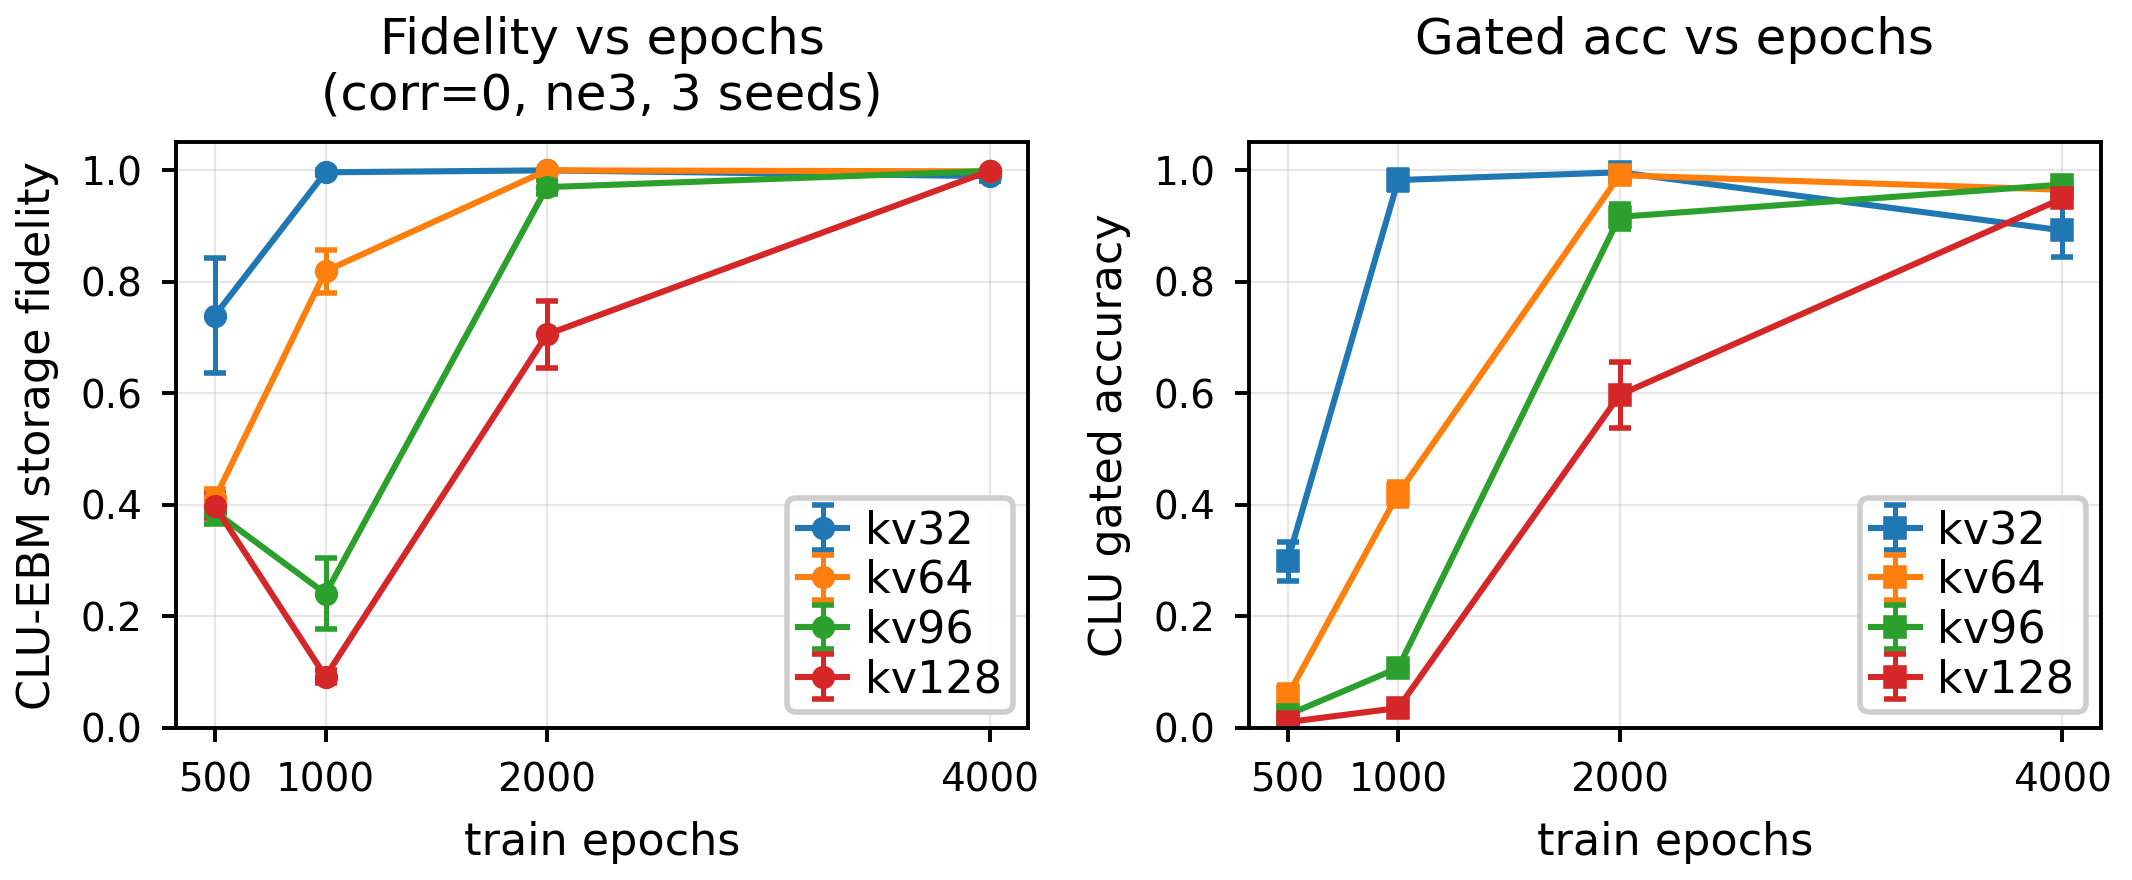
\includegraphics[width=0.82\linewidth]{figs/fig_frontier_clean.png}
\caption{\textbf{Epoch-scaling frontier:} CLU-EBM
storage fidelity and gated accuracy against training budget for kv$\in\{32,64,96,128\}$.
Required epochs scale with capacity rather than saturating at a fixed ceiling, and kv$32$
over-trains between $2000$ and $4000$ epochs.}
\label{fig:frontier}
\end{figure}

\section{Discussion}
We establish that on a CLU-like conservative memory, test-time compute is certified access: the phase-volume, energy and latch consequences of every access mechanism are fixed by the dynamics. A squeeze cures escape with a bounded energy injection but requires energy growing exponentially in rapidity $\zeta$, and therefore quadratically in the excess distance, whereas a non-local gated channel achieves global reach at exact volume preservation ($\detJ=1$), an energy requirement that is fixed and independent of distance (exactly zero on the matched channel measured here), and strictly preserved latch transport. We note that while these certificates govern the physical transport of the memory state, bounding the energy change is an insufficient condition for BIBO stability; strict coercive-component screening is required. Empirically, these mechanisms facilitate scalable internal compute rationing on clean retrieval tasks for CLU-like units.

Furthermore, we identify an impossibility result regarding the memory read protocol. With a quadratic payload channel and a fixed read budget, a store cannot simultaneously possess exact value fidelity, amplitude-independent address hold, and amplitude-independent read latency. The implementation must sacrifice one of these properties, dictating that a faded memory mathematically requires more integration steps to read. Our future work includes probing learned entrance-steering for the gated channels, retry acceptance as a certified kernel and evaluation of our methods on learned latent potentials at scale.

\bibliographystyle{plainnat}
\bibliography{refs}

\appendix

\section{Contributions}
\label{app:contri}
\begin{enumerate}\itemsep2pt
\item \textbf{Formalization of failure modes:} We partition reachability failures into kinematic reach, where the target lies outside a causal box $C_T$ bounded by $L_i=T\varepsilon c/\sqrt{M_i}$, and energetic escape, where the target is inside $C_T$ but shielded by a potential barrier. These are resolved by distinct mechanisms carrying different certificates.
\item \textbf{Verification of the certificate stack:} We verify our theoretical predictions on an analytic testbed using dimensions 2 and 4, 5 seeds, and oracle placement. We confirm that the Lorentz squeeze cures escape with bounded injection and extends reach at an energy exponential in the rapidity. We also verify that the gated channel mechanism cures reach continuously with $\detJ=1$, a fixed energy change exact to zero, and exact latch transport.
\item \textbf{Empirical measurement of latch transport:} We demonstrate that an untrained state-replacing map has $\detJ=0$ exactly, resulting in the complete erasure of stored Goldstone charge. In contrast, the certified gated channel transports the charge with preserved spread. We explicitly establish that phase volume alone is insufficient for this transport; a matched channel is required. Furthermore, a bounded energy change is necessary but insufficient for Bounded-Input Bounded-Output (BIBO) stability without coercive-component screening.
\item \textbf{Memory-agnostic calibrated compute-rationing:} We implement a self-calibrating compute-rationing gate on an escalatable learned memory. We observe a $4.81\pm0.44\times$ reduction in relaxation steps at the kv16 capacity level at a 400-epoch budget. The primary asset is escalatability and rationing rather than baseline energy signal superiority, and the gating mechanism itself is memory-agnostic.
\item \textbf{Scaling boundaries for non-local routing:} We verify that a direct one-hop non-local edge demonstrates a flat FLOP count under distance scaling relative to multi-hop diffusion. However, we explicitly report that energy-gating this mechanism is outperformed by a parameter-matched, physics-free router in both floating-point operations (FLOPs) and accuracy.
\item \textbf{Capacity and epoch-budget map of the compute dial:} We map the rationing gate across capacity and training budget. The measured step-reductions ($9.9\times, 9.5\times, 6.2\times$ across kv32, kv64, kv96) are intra-CLU rationing against a full-budget CLU baseline, performance beyond kv64 is constrained by epoch-budgets rather than hard capacity limits, and gate accuracy degrades sharply under evaluation cue noise while storage fidelity remains at $1.0$.
\end{enumerate}
The primary contribution of this work lies in the theoretical formalization of the certificate stack and the empirical discipline mapping its limitations, rather than claiming a general leaderboard advantage. All computational experiments were conducted on standard laptop CPUs.

\section{Flag-Provenance Tables}
All computational results inherit the exact non-default configurations in effect.

\subsection{Certificate Stack Configuration}
\noindent{\footnotesize
\begin{tabular}{@{}p{0.24\textwidth}p{0.70\textwidth}@{}}
\toprule
Flag & Value \\
\midrule
% Theory commit & \texttt{9a13455} (analytic checks, numpy float64, \texttt{default\_rng(0)}) \\
% Experiment commit & \texttt{6f2384c} \\
JAX & 0.9.0 \\
Kinetic modes & relativistic (reach, gated channel, throat); \texttt{newtonian\_learned} (Newtonian control) \\
Mass band & $[4.0, 0.25]$ yielding $M_{\rm eff,0}=4.0$, $16\times$ contrast \\
$c$ / rest mass / $m_0$ & 1.0 / 1.0 / 1.0 \\
Time step dt / Horizon $T$ & 0.05 / 100 yielding box $L=T\varepsilon c/\sqrt{M_0}=2.5$, $v_{\max,0}=0.5$ \\
Damping $\gamma$ & reach rollout $\gamma=0$ (sharp box) \\
Rapidity $\zeta$ grid & $[0,0.1,0.2,0.3,0.4,0.6,0.8,1.0,1.5,2.0]$ \\
Basin geometry & double well along coord 0, barrier $\Delta V_b=1.0$, $d\in\{0.8,1.6,2.4,3.2,4.0,5.0\}$ \\
Initialization & $q_0=0$, $p_0=(1.2,0,\dots)+0.02\,\mathcal N$ (kinetic energy below barrier) \\
Landing criterion & $\min_{\rm traj}|q_0-d|<0.4$ \\
Seeds & reach $\{0,1,2,3,4\}$; latch \texttt{default\_rng(0)} \\
Dimensions & 2 and 4 \\
\bottomrule
\end{tabular}}

\subsection{Calibrated Gate Configuration}
\noindent{\footnotesize
\begin{tabular}{@{}p{0.24\textwidth}p{0.70\textwidth}@{}}
\toprule
Flag & Value \\
\midrule
% Commit & \texttt{572c708} \\
Task & MQAR CLU-EBM, vocab 256, capacity kv$\in\{16,24,32\}$ \\
Seeds & 5 (base 42); 90 models \\
Write configuration & kinetic relativistic, potential mlp, hidden 128, epochs 400, lr $1\mathrm{e}{-3}$, batch 16, k\_steps 50, buffer 128, friction 0.3, temperature 0.3, input noise $\sigma$ 0.05 \\
Gate configuration & calib features \texttt{r\_margin}, learned $\tau$ at write time, $p_{\rm exit}=0.5$; cost checkpoints $300/1200/2100/3000$ \\
Learn-then-Test & fixed-sequence, exact binomial p-values, targets $\varepsilon\in\{0.05,0.1\}$ \\
Hopfield baseline & Platt-calibrated logit margin, identically probed \\
\bottomrule
\end{tabular}}

\subsection{Routing Configuration}
\noindent{\footnotesize
\begin{tabular}{@{}p{0.24\textwidth}p{0.70\textwidth}@{}}
\toprule
Flag & Value \\
\midrule
% Commit & \texttt{52330f8} \\
Lattice and task & distance $N\in\{4,8\}$, embed\_dim 12, vocab 128 \\
Write configuration & kinetic relativistic, potential mlp (coercive), hidden 128, epochs 400, lr $1\mathrm{e}{-3}$ \\
Retrieval routing & dt 0.05, relax\_steps 250, governor\_sensitivity 0.95 \\
Router MLP & hidden 32 (449 params), epochs 300, lr $3\mathrm{e}{-3}$ \\
Workload mixes & $[[0.5,0.5],[0.8,0.2],[0.95,0.05]]$ \\
\bottomrule
\end{tabular}}

\subsection{Regime Map Configuration}
\noindent{\footnotesize
\begin{tabular}{@{}p{0.24\textwidth}p{0.70\textwidth}@{}}
\toprule
Flag & Value \\
\midrule
% Commit & \texttt{63fea62} \\
Training epochs & swept across $\{500,1000,2000,4000\}$ \\
Kinetic and potential & relativistic / mlp (coercive) \\
Architecture & embed\_dim 16 (CLU dim 32) / hidden 128 / vocab 256 \\
Retrieval & relax\_steps 300, governor\_sensitivity 0.95, calib \texttt{r\_margin} \\
Seeds & $\{42,43,44,45,46\}$ \\
\bottomrule
\end{tabular}}

\subsection{Latch Transport and BIBO Battery Configuration}
\noindent{\footnotesize
\begin{tabular}{@{}p{0.24\textwidth}p{0.70\textwidth}@{}}
\toprule
Flag & Value \\
\midrule
% Commit & \texttt{27f232f} \\
Training & none; analytic potentials, oracle channel placement \\
Kinetic mode & relativistic (reach, gated channel, throat, BIBO) \\
Damping $\gamma$ & reach 0 (sharp box); BIBO 0.02 (bounded arms must settle) \\
BIBO potential & $k=1.0$, $\epsilon=0.02$ yielding $x_b=3.5355$, barrier $V_b=3.125$ \\
BIBO parameters & exits $b\in\{1.0,2.0,3.0,3.6,4.0,5.0\}$; horizon $T=2000$ \\
Latch transport & 16 incoming states, ball radius $0.3<\rho=0.35$ \\
Seeds & reach/BIBO $\{0,1,2,3,4\}$; latch cloud \texttt{default\_rng(0)} \\
\bottomrule
\end{tabular}}

We note that the two primary configuration axes influencing comparative performance are damping and training epochs. The calibrated gate evaluation utilizes $\gamma=0.3$ and 400 epochs, capturing an under-converged regime. In contrast, the regime mapping sweeps up to 4000 epochs to isolate converged behavior.

\section{The Access-Certificate Table and BIBO Battery}
\subsection{Table 1: Certificate per Mechanism}
\begin{center}\footnotesize
\begin{tabular}{p{2.6cm}p{2.3cm}p{1.8cm}p{3.0cm}p{2.5cm}}
\toprule
Mechanism & Energy Injected & Volume $\detJ$ & Governor Re-absorption & Latch Impact \\
\midrule
Gated channel (translation) & $\Delta V{=}V(b){-}V(a)$, discrete jump & 1 exactly & $\approx(1/\gamma_c)\ln(1{+}\Delta V/E^\star)$ & Transport via shift $p^\top X\Delta$ \\
Gated channel (throat) & standing wave, no jump & $(1{-}\gamma)^d$ exact & continuous & adds $\mu^2{\propto}A/\ell^2$ \\
Squeeze $S^{(M)}$ & $\le(e^{2|\zeta|}{-}1)H$ & 1 exactly & $\approx2\zeta/\gamma_c$ & preserved \\
\bottomrule
\end{tabular}
\end{center}
Both jump mechanisms mandate evaluation alongside a coercive potential $V_\theta$. Because deep convolutional potentials are architecturally non-coercive out-of-unit, exits must be strictly constrained to lie inside a coercive sub-level component.

\subsection{The BIBO Battery}
\begin{figure}[t]\centering
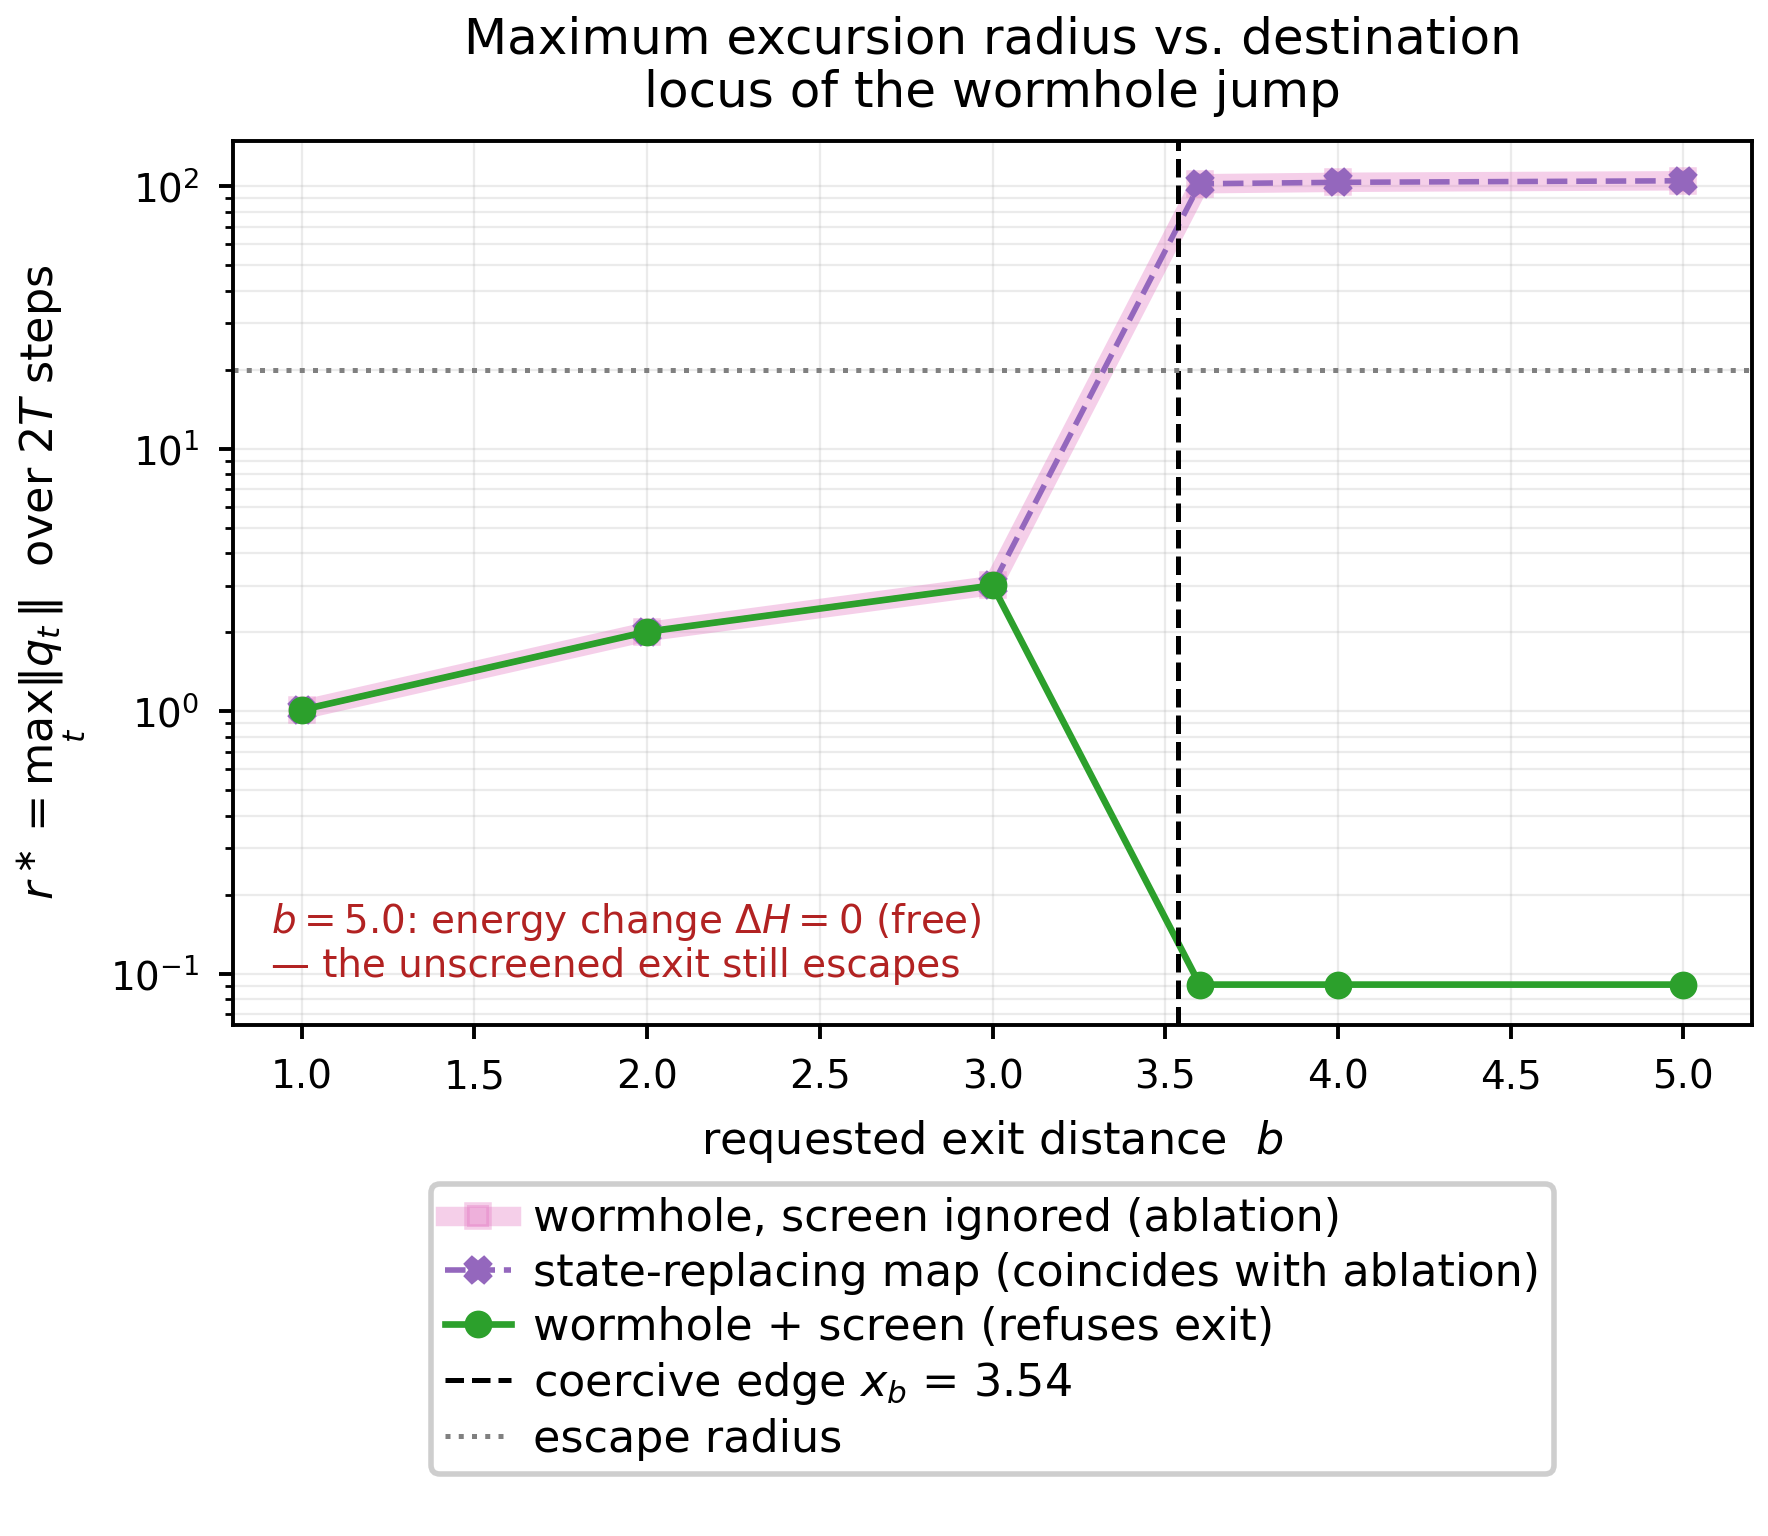
\includegraphics[width=0.68\linewidth]{figs/fig4_bibo.png}
\caption{\textbf{The BIBO battery:} Maximum excursion radius
$r^\ast=\max_t\|q_t\|$ at horizon $2T$, against the requested exit locus $b$. Exits inside the
coercive component stay bounded for every arm. Beyond the coercive edge $x_b=3.54$ the
unscreened arms grow as $r^\ast\propto T$, while the screened gated channel holds at $r^\ast=0.09$
because it \emph{refuses} the jump rather than making it safe. The state-replacing map
coincides exactly with the screen-ignored ablation, so what provides boundedness is the screen and
not the jump. Note $b=5.0$: the energy change is exactly zero and the exit still escapes.}
\label{fig:bibo}
\end{figure}
We evaluate the bounding capabilities on a controlled non-coercive well where the connected component spans $|q_0|<x_b=3.536$. We assess the maximum excursion radius $r^\ast$ at horizons $T$ and $2T$.

\begin{center}\small
\begin{tabular}{lcccccc}
\toprule
Algorithm ($r^\ast$ at $2T$) & $b{=}1.0$ & $2.0$ & $3.0$ & $3.6$ & $4.0$ & $5.0$ \\
\midrule
Gated channel with certificate & $1.01$ & $2.01$ & $3.01$ & $0.09$ & $0.09$ & $0.09$ \\
Gated channel, ablation & $1.01$ & $2.01$ & $3.01$ & $102.13$ & $103.43$ & $104.83$ \\
State-replacing map & $1.01$ & $2.01$ & $3.01$ & $102.13$ & $103.43$ & $104.83$ \\
\midrule
Escape rate, certified & $0$ & $0$ & $0$ & $0$ & $0$ & $0$ \\
Escape rate, blind & $0$ & $0$ & $0$ & $1.0$ & $1.0$ & $1.0$ \\
Gated channel certificate logic & ADMIT & ADMIT & ADMIT & REJECT & REJECT & REJECT \\
Energy sub-level test & admit & admit & admit & reject & admit & admit \\
\bottomrule
\end{tabular}
\end{center}

The escaping arms present a linear growth rate $r^\ast(2T)/r^\ast(T)\approx1.9$, demonstrating genuinely unbounded trajectories constrained only by the terminal velocity cap. The critical evaluation occurs at exit $b=5.0$, where the energy change is exactly zero, causing an energy-only sub-level test to erroneously admit the jump, resulting in immediate escape. This conclusively demonstrates that $\detJ=1$ combined with a zero energy change is insufficient for BIBO stability; coercive-component membership is the requisite property. Furthermore, the blind gated channel and state-replacing maps coincide exactly on all failures, proving that the certificate screening mechanism, not the jump itself, provides the bounding guarantee.

\section{Evaluation Results}
\label{app:res}

\subsection{Verification of the Certificate Stack}
\label{sec:certificates}
To empirically validate the certificates, we employ an architecturally-invariant, small-scale analytic testbed. The environment consists of a symmetric double well along the reach coordinate and an $SO(2)$ sector for the latch. All results in this section are evaluated across latent dimensions 2 and 4, utilizing 5 random seeds, designed channel placement, single-CPU execution, a sharp boundary $\gamma=0$ rollout, and a mass band of $[4.0,0.25]$ to yield a $16\times$ inertial contrast. This controlled setting isolates the exactness of the physical theory; learning optimal entrance placement remains outside the current scope.

The squeeze requires more energy than the swept rapidity grid provides at $d=4.0$. The mathematical bracket accurately predicts that reaching $d=4.0$ requires a rapidity of $\zeta\ge2.0105$, corresponding to an energy bound growing as $e^{2|\zeta|}$ in the rapidity. The state-replacing map is an untrained analytic constant map with $\detJ=0$ exactly, distinct from the learned decision head evaluated in the routing section.

The validation of the squeeze at varying rapidities: $(\zeta,\text{ratio},\text{bound})=(0.25,1.13,1.65), (0.5,1.55,2.72), (1.0,3.79,7.39), (2.0,27.5,54.6)$, while strictly maintaining $\det S^{(M)}=1.000\ (\pm4\times10^{-6})$. We note that the $e^{2|\zeta|}$ bound is a matched-quadratic certificate; applied to a quartic well, the raw ratio can naturally exceed this limit.

The gated channel is evaluated on the symmetric double well with channel $-a\to+a$, the exact energy change evaluates to $0.0$, successfully translating the state to $q=+1.000$ with $\detJ=1.000$.

The Goldstone charge is strictly preserved if and only if $\Delta\perp X^\top p$; otherwise, it shifts by precisely $p^\top X\Delta$. We empirically observe a zero-shift $\Delta Q=0.0$ (predicted precision $7.5\times10^{-10}$) and an across-coset shift of $\Delta Q=0.2500=p^\top X\Delta$. A random baseline shift entirely erases the latch. The matched channel, defined as $\Delta$ being coset-tangent alongside the energy constraint, guarantees stable transit.

\begin{center}\footnotesize
\begin{tabular}{lcccccc}
\toprule
Mechanism & $\detJ$ & $\Delta Q$ mean & $\Delta Q$ std & Predicted $p^\top X\Delta$ & Max Error & $\mathrm{std}(Q_{\rm out})$ \\
\midrule
Gated channel (coset-tangent) & $1.0000$ & $-0.0000$ & $0.0000$ & $0.0000$ & $1.2\mathrm{e}{-7}$ & $0.0803$ \\
Gated channel (across-coset) & $1.0000$ & $0.2500$ & $0.0000$ & $0.2500$ & $0.0$ & $0.0803$ \\
Random shift & $1.0000$ & $0.0972$ & $0.2465$ & \emph{N/A} & --- & $0.2793$ \\
State-replacing map & $0.0000$ & $0.0379$ & $0.0803$ & \emph{N/A} & --- & $0.0$ \\
\bottomrule
\end{tabular}
\end{center}

\subsection{Reach Battery Full Grid}
Evaluated across 5 seeds with causal box $L=2.5$.
\begin{center}\footnotesize
\begin{tabular}{lcccccc}
\toprule
Algorithm & $d{=}0.8$ & $1.6$ & $2.4$ & $3.2$ & $4.0$ & $5.0$ \\
\midrule
Plain relaxation & 0 & 0 & 0 & 0 & 0 & 0 \\
Squeeze $S^{(M)}$ & 1 & 1 & 1 & 1 & 0 & 0 \\
Gated channel & 1 & 1 & 1 & 1 & 1 & 1 \\
Newtonian control & 1 & 1 & 1 & 1 & 1 & 1 \\
State-replacing map & 1 & 1 & 1 & 1 & 1 & 1 \\
Dense/$V$-throat & 1 & 0.8 & 0 & 0 & 0 & 0 \\
\bottomrule
\end{tabular}
\end{center}

\subsection{Routing Full Grid}
Evaluated across 5 seeds for local and distant accuracy (L/D) and floating-point operations per query.
\noindent{\footnotesize
\begin{tabular}{@{}lcccc@{}}
\toprule
Algorithm & $N{=}4$ Acc (L/D) & $N{=}4$ FLOP & $N{=}8$ Acc (L/D) & $N{=}8$ FLOP \\
\midrule
Local only & $0.500$ ($1.00$/$0.00$) & $5.88\mathrm{e}7$ & $0.500$ ($1.00$/$0.00$) & $5.88\mathrm{e}7$ \\
Gated energy & $0.887\pm0.139$ ($0.90$/$0.88$) & $1.18\mathrm{e}8$ & $0.715\pm0.172$ ($0.82$/$0.61$) & $1.18\mathrm{e}8$ \\
Dense network & $0.500$ ($0.00$/$1.00$) & $1.18\mathrm{e}8$ & $0.448\pm0.070$ ($0.00$/$0.90$) & $1.18\mathrm{e}8$ \\
Diffusion chain & $0.652\pm0.159$ ($0.90$/$0.41$) & $1.76\mathrm{e}8$ & $0.548\pm0.138$ ($0.82$/$0.28$) & $2.94\mathrm{e}8$ \\
Physics-free router & $1.000\pm0.000$ ($1.00$/$1.00$) & $8.81\mathrm{e}7$ & $0.948\pm0.070$ ($1.00$/$0.90$) & $8.81\mathrm{e}7$ \\
\bottomrule
\end{tabular}}

\begin{center}\footnotesize
\begin{tabular}{lccccc}
\toprule
Cell (N,kv) & Epochs & CLU Fidelity & Gate Acc & Intra-CLU Step-Reduction \\
\midrule
N128/kv32 & 500 & $0.76\pm0.09$ & $0.31\pm0.04$ & $1.2\times$ \\
N128/kv32 & 2000 & $1.00\pm0.00$ & $1.00\pm0.00$ & $9.9\times$ \\
N256/kv64 & 500 & $0.43\pm0.05$ & $0.06\pm0.02$ & $1.0\times$ \\
N256/kv64 & 2000 & $1.00\pm0.00$ & $0.99\pm0.00$ & $9.5\times$ \\
N384/kv96 & 500 & $0.40\pm0.03$ & $0.02\pm0.01$ & $1.0\times$ \\
N384/kv96 & 2000 & $0.97\pm0.01$ & $0.91\pm0.02$ & $6.2\times$ \\
\bottomrule
\end{tabular}
\end{center}

The epoch-scaling frontier confirms that required epochs scale with capacity. While kv32 saturates by 1000 epochs, kv96 requires 4000 epochs to achieve an accuracy of $0.975$. We explicitly observe over-training artifacts where smaller cells degrade when trained to excessive horizons.

\section{Documented Negative Results}
We explicitly record several primary negative findings to demarcate the boundaries of our mechanisms. First, the squeeze retries recover no performance at a single-unit scale when selecting among already reachable attractors, demonstrating that the squeeze addresses kinematic reach failure rather than local selection. Second, the compute dial does not confer robustness to corrupted cues: gate accuracy degrades sharply under evaluation cue noise while storage fidelity remains perfect, indicating that the governed relaxation over-commits to the corrupted cue rather than failing to store the pattern. Noise-aware thresholds, longer relaxation budgets and denoising initialization are open work. Finally, we confirm that the raw energy signal adds negligible predictive value over a standard readout margin, establishing that our framework relies on the calibrated rationing mechanism itself rather than an inherently superior physics signal.

\section{Analytic Verification Protocols}
All verifications were conducted using standard numerical precision implementations in Python on CPU architectures. The reach causal cap was validated to a relative error of $2.0\times10^{-12}$. The Jacobian preservation was validated to $1.000$, with state-dependent variations correctly tracking the expected analytical deviations to $2.2\times10^{-16}$. The Goldstone latch transit error remained bounded below $1.8\times10^{-15}$. Finally, the governor re-absorption mechanics accurately tracked the theoretical exponential injections across all swept rapidities.

\section{Derivations for Certified Markov Kernels}
To secure a stationarity certificate for test-time retries, we derive the four operating constraints for the proposed Markov kernel. First, because the symmetric Lorentz squeeze is exactly volume-preserving ($\detJ=1$), it requires no Jacobian correction in the acceptance ratio. A retry proposing a sign-symmetrized squeeze and accepting via $\min(1,e^{-\Delta H/T})$ forms a detailed-balance kernel for $e^{-H/T}$ \citep{duane_hybrid_1987}. However, because the state-dependent governor constitutes non-volume-preserving dissipation, the deployed sequence is effectively Metropolis-within-annealing, converging to a colder maximum-a-posteriori state rather than acting as a pure Gibbs sampler.

Second, the squeeze family orbit represents a single hyperbola, rendering it non-ergodic. Ergodicity strictly necessitates momentum refreshment, requiring the squeeze to be layered with a Metropolis-Adjusted Langevin Algorithm step to ensure proper mixing across the state space \citep{brooks_mcmc_2011}.

Third, the Langevin noise scale must be calibrated using the discrete fluctuation-dissipation relation, defined as $\sigma_i^\star=\sqrt{M_{{\rm eff},i}T\gamma(2-\gamma)}$ \citep{roberts_exponential_1996}. Applying the correct calibration reduces the shadow bias finite-budget error from $0.0995$ to $0.0065$. In relativistic kinetic modes, the target distribution follows Maxwell-J\"uttner statistics; therefore, fixed-covariance Gaussian refreshes are invalid, and stationarity is solely maintained by the Metropolis-Hastings corrections.

Finally, because the Gibbs measure is uniformly flat along Goldstone cosets, any coset-tangent proposal has an energy differential of zero and is accepted uniformly. This dynamic generates an unbiased random walk that diffuses and erodes the stored register at a rate proportional to the proposal scale variance. Explicit projection orthogonal to the coset tangent successfully quenches this drift, proving that without projection, even a certified MCMC retry mechanism will progressively erase stored memory contents.

\section{Derivations for the Reach and Injection Certificates}
\label{app:deriv}
This appendix derives the two closed forms the main text relies on the causal box and the bounded-injection certificate $H(S_\zeta z)\le e^{2|\zeta|}H(z)$ together with the hard-gate Jacobian. Everything follows from the governed map. Throughout, $z=(q,p)\in\R^d\times\R^d$, and in relativistic mode the reference architecture's kinetic energy is
\[
T(p)=\sqrt{c^2\,p^\top M^{-1}p+m_0^2c^4},
\]
with $M=\mathrm{diag}(M_1,\dots,M_d)\succ0$ the learned inertial mass and $m_0>0$ the rest mass (values in the flag table).

\subsection{The causal box}
\label{app:deriv:box}
\paragraph{Claim.}
One drift sub-step advances each coordinate by strictly less than $\varepsilon c/\sqrt{M_i}$, for every momentum $p$ and every potential $V_\theta$; consequently $Q_T(z_0)\subseteq C_T(q_0)$ with $L_i=T\varepsilon c/\sqrt{M_i}$.

\paragraph{Derivation:}
The drift sub-step of the kick--drift--kick map moves only the position, $q\mapsto q+\varepsilon\,\nabla_pT(p)$, at whatever momentum is current at that sub-step. Differentiating $T$,
\[
\frac{\partial T}{\partial p_i}=\frac{c^2p_i}{M_i\,T(p)},
\qquad
T(p)=\Bigl(c^2\sum\nolimits_j p_j^2/M_j+m_0^2c^4\Bigr)^{1/2}>\frac{c\,|p_i|}{\sqrt{M_i}},
\]
the last inequality strict for every $p$ because $m_0>0$ and the remaining kinetic terms are non-negative. Hence
\[
|\dot q_i|=\Bigl|\frac{\partial T}{\partial p_i}\Bigr|=\frac{c^2|p_i|}{M_i\,T(p)}<\frac{c^2|p_i|}{M_i}\cdot\frac{\sqrt{M_i}}{c\,|p_i|}=\frac{c}{\sqrt{M_i}},
\]
so a single drift obeys $|q_i'-q_i|<\varepsilon c/\sqrt{M_i}$. The two kick sub-steps and the damping $p\mapsto(1-\gamma)p$ act on momentum only and move no position, so the same bound holds for the full step, uniformly in $\theta$, $\gamma$, and the state. Summing over $n\le T$ steps gives $|q_{n,i}-q_{0,i}|<n\varepsilon c/\sqrt{M_i}\le L_i$, i.e.\ $Q_T(z_0)\subseteq C_T(q_0)$.

\paragraph{Energy-blindness:}
The bound involves only $(\varepsilon,c,M_i)$: neither $V_\theta$ nor the magnitude of $p$ enters. Injected momentum drives $|\dot q_i|$ toward the cap from below, with relative deficit $1-|\dot q_i|\sqrt{M_i}/c\approx m_0^2c^2M_i/(2p_i^2)$ as $|p_i|\to\infty$ (momentum along coordinate $i$) the saturation. With the stated configuration ($T=100$, $\varepsilon=0.05$, $c=1$, $M_0=4.0$) the reach coordinate has $L=2.5$ and $v_{\max,0}=0.5$. In Newtonian mode $\nabla_pT=M^{-1}p$ is unbounded, no such box exists, and reach is energy-limited, which is why the Newtonian control crosses the box.

\subsection{The bounded-injection certificate}
\label{app:deriv:squeeze}
\paragraph{The map.}
On the targeted coordinate pair $(q_i,p_i)$, pass to mass-weighted coordinates $u=\sqrt{M_i}\,q_i$, $v=p_i/\sqrt{M_i}$ and let the mass-weighted squeeze $S^{(M)}_\zeta$ act as the hyperbolic rotation
\[
u'=u\cosh\zeta+v\sinh\zeta,\qquad v'=v\cosh\zeta+u\sinh\zeta,
\]
identity on all other coordinates. In the original variables, $q_i'=q_i\cosh\zeta+(p_i/M_i)\sinh\zeta$ and $p_i'=p_i\cosh\zeta+M_iq_i\sinh\zeta$. The map is linear with determinant $\cosh^2\zeta-\sinh^2\zeta=1$ on the active pair and $1$ elsewhere, hence exactly symplectic: this is the $\det S^{(M)}=1$ certificate.

\paragraph{Displacement law and the reach bracket:}
Applied at the launch state of the reach battery ($q=0$, momentum $p_0$ along the heavy coordinate), the squeeze produces the instantaneous displacement $q_0'=(p_0/M_0)\sinh\zeta$; the subsequent governed flow advances by at most the box half-width $L$ (Appendix~\ref{app:deriv:box}). The squeeze-extended reach is therefore contained in the bracket $[\,L,\;L+p_0\sinh\zeta/M_0\,]$ of Figure~\ref{fig:reach}. Landing at distance $d$ within the tolerance $0.4$ of the flag table requires $(p_0/M_0)\sinh\zeta\ge d-0.4-L$, i.e.
\[
\zeta\ \ge\ \operatorname{arcsinh}\!\bigl((d-0.4-L)\,M_0/p_0\bigr),
\]
which at $L=2.5$, $p_0=1.2$, $M_0=4.0$ evaluates to $\zeta\ge2.0105$ for $d=4.0$ and $\zeta\ge2.64$ for $d=5.0$. Both exceed the swept budget $\zeta\le2.0$, which is why the squeeze row of the reach battery drops to zero at $d\ge4.0$ while $d\le3.2$ remains covered.

\paragraph{The energy bound:}
The certificate is a matched-quadratic statement: on the active pair the quadratic Hamiltonian is isotropic in the same mass-weighted coordinates, $H_{\mathrm q}=\half\kappa\,(u^2+v^2)$ with $\kappa>0$. Under the squeeze,
\[
u'^2+v'^2=(u^2+v^2)\cosh2\zeta+2uv\,\sinh2\zeta
\ \le\ (u^2+v^2)\bigl(\cosh2\zeta+|\sinh2\zeta|\bigr)
=(u^2+v^2)\,e^{2|\zeta|},
\]
using $2|uv|\le u^2+v^2$. Hence $H(S_\zeta z)\le e^{2|\zeta|}H(z)$, with equality exactly on the diagonal $u=\pm v$ (sign matched to that of $\zeta$), and the injected energy obeys $\Delta H\le(e^{2|\zeta|}-1)H$, the form quoted in the certificate table. Spectator coordinates only tighten the bound: they contribute the same non-negative energy to both sides and pull the ratio toward one. Two consequences used in the text: at the launch state $u=0$ the ratio equals $\cosh2\zeta$ exactly, so the measured ratios must lie between $\cosh2\zeta$ and the bound $e^{2|\zeta|}$, as they do; and the bound is attained only on the diagonal, so generic states sit strictly below it.

\paragraph{Exponential in rapidity, quadratic in excess distance:}
Writing $\delta=(p_0/M_0)\sinh\zeta$ for the displacement beyond $L$, the launch-state ratio is
\[
\cosh2\zeta=1+2\sinh^2\zeta=1+2\,(M_0\delta/p_0)^2,
\]
exactly quadratic in $\delta$, while the certificate $e^{2|\zeta|}=(\cosh\zeta+|\sinh\zeta|)^2$ is exponential in the rapidity and likewise quadratic in $\delta$ at large $\zeta$. This is the scaling stated in the abstract; the energy is \emph{not} exponential in the distance itself.

\paragraph{Scope:}
The inequality is proved for the matched quadratic $H$. On a quartic well the potential term transforms with higher powers of $\cosh\zeta$, so the raw ratio can exceed $e^{2|\zeta|}$, exactly as reported.

\subsection{The hard-gate Jacobian}
\label{app:deriv:gate}
\paragraph{Claim:}
If the gate is allowed to vary during the jump, $q\mapsto q+g(q)\Delta$, $p\mapsto p$, then $\detJ=1+\nabla g(q)\cdot\Delta$; freezing the gate at capture ($g$ constant during the jump) restores $\detJ=1$ exactly.

\paragraph{Derivation:}
The Jacobian is block-triangular with momentum block $I_d$ and position block the rank-one update $\partial q'/\partial q=I_d+\Delta\,\nabla g(q)^\top$, so by the matrix determinant lemma
\[
\detJ=\det\bigl(I_d+\Delta\,\nabla g(q)^\top\bigr)=1+\nabla g(q)^\top\Delta.
\]
The defect is first order in the gate's variation along the jump, so no smallness of $\Delta$ removes it (unit-test value $2.05$).

\section{Design rules for certified Markov kernels:}
The MCMC implementation necessitates four strict design rules. First, because the state-dependent governor constitutes non-volume-preserving dissipation, the actual cascade operates as Metropolis-within-annealing; we do not claim stationarity for the governed composite. Second, because the squeeze family orbit is reducible and non-ergodic, it must be layered onto a Metropolis-Adjusted Langevin Algorithm (MALA) step \citep{roberts_exponential_1996} to ensure adequate mixing. Third, the Langevin noise scale must be calibrated using the discrete fluctuation-dissipation relation to prevent finite-budget shadow bias. Finally, because the Gibbs measure is uniformly flat along Goldstone cosets, random walk drift will erode the stored memory register. Explicit projection orthogonal to the coset tangent is strictly required to prevent topological degradation.

\end{document}
